\section{Návrh strategické hry}

\begin{itemize}
    \item Představení cíle kapitoly.
    \item Vysvětlení, proč je důležité systematicky navrhnout jednotlivé prvky hry.
    \item Úvodní představy
    \begin{itemize}
        \item Herní koncept (typ hry, pravidla, cíle hráče).
        \item Popis mapy: Použití dlaždic a jejich vliv na herní mechaniky.
    \end{itemize}
    \item Odkaz na \textit{The Art of Game Design} a použitý rámec návrhu.
    \item Přehled toho, co bude v kapitole popsáno.
\end{itemize}

Zpracováno na základě: \cite{} \cite{} \cite{}.

V této kapitole rozeberu postup návrhu jednoduché strategické hry hrané na náhodně vygenerované mapě.

Návrh strategické hry vyžaduje systematický přístup k definování jejích klíčových prvků. Aby byla hra hratelná, vyvážená a pokud možno i zábavná, je zapotřebí systematicky rozebrat a promyslet návrh všech částí hry. 

Základní představa, se kterou jsem začínal před samotným systematickým návrhem, byla taková, že hra bude 2D tahová strategie s prvky správy surovin. Hráči budou ovládat a vylepšovat své jednotky, spravovat zdroje a budovat infrastrukturu, přičemž se budou snažit dosáhnout vítězství nad soupeřem. Herní svět je reprezentován dlaždicovou mapou, typ terénu na dlaždici ovlivňuje pohyb jednotek, možnosti výstavby a dostupnost zdrojů.

Pro návrh hry využívám metodologii z knihy \textit{The Art of Game Design: A Book of Lenses} od Jesseho Schella, která strukturuje herní design do několika klíčových kategorií:

\begin{itemize}
    \item Prostor -- Jak je herní svět uspořádán a jak se v něm hráči pohybují.
    \item Objekty, atributy a stavy -- Jaké herní entity existují, jaké mají vlastnosti a jaké stavy mohou při hře nastat.
    \item Akce hráče -- Jaké interakce může hráč provádět a jak ovlivňují hru.
    \item Pravidla hry -- Jaké jsou omezení a podmínky vítězství.
    \item Dovednost a náhoda -- Jaký je poměr mezi strategickým rozhodováním a prvky náhody.
\end{itemize}

Tento rámec poskytuje ucelený pohled na návrh hry a pomáhá zajistit, aby všechny prvky dohromady tvořily soudržný a dobře vyvážený celek.

Ve zbytku kapitoly rozeberu podrobněji právě tyto herní prvky a konkretizuji herní návrh.

\subsection{Prostor}
\begin{itemize}
    \item Struktura herního světa a jeho reprezentace.
    \item Herní mapa:
    \begin{itemize}
        \item Dlaždicová struktura a její výhody.
        \item Typy terénu a jejich vlastnosti.
    \end{itemize}
    \item Pohyb pouze ve čtyřech směrech
\end{itemize}

Každá hra obsahuje nějaký herní prostor, ve kterém se celá hra odehrává. Ten obecně vymezuje herní lokace a určuje, jak jsou mezi sebou propojeny. Z pohledu herních mechanik považujeme prostor za matematickou konstrukci, tedy je potřeba odfiltrovat veškeré vizuální prvky a zaměřit se pouze na abstraktní uspořádání prostoru.

Kniha \textit{The Art of Game Design: A Book of Lenses} rozděluje herní prostory podle několika parametrů:

\begin{itemize}
    \item Diskrétnost vs. kontinuita -- Prostor může být buď diskrétní, nebo kontinuální. Diskrétní prostor je tvořen pevně stanovenými, oddělenými místy, kontinuální prostor umožňuje pohyb v plynulém, nekonečném rozsahu.
    \item Počet dimenzí -- Každý herní prostor má určitý počet dimenzí, které definují jeho rozsah a strukturu. Prostor může být jednorozměrný, dvourozměrný nebo dokonce třírozměrný, jak ukazuje například herní stůl na kulečník.
    \item Ohraničenost a propojení oblastí -- Prostor může být uzavřený, s pevně definovanými hranicemi, nebo otevřený, umožňující pohyb hráče nebo herních prvků mimo hranice. Rovněž je důležité zvážit, zda jsou jednotlivé části prostoru propojené, nebo zda jsou oddělené a nezávislé.
\end{itemize}

Příklad hry hrané na diskrétním dvoudimenzionálním poli je "piškvorky" (v rámci příkladu předpokládám herní plochu $3\times3$), kde herní plocha je rozdělena na devět oddělených políček. Herní deska je zobrazena jako souvislý prostor, ale z hlediska herních mechanik bereme v potaz pouze těchto devět specifických míst, která můžeme znázornit jako uzly v síti. Tedy dokud je jednoznačně rozeznatelné, do kterého políčka zapadá, jsou si mechanicky ekvivalentní, jak je naznačeno na obrázku \ref{sudoku}.

\begin{figure}
  \centering      % vycentrovat
  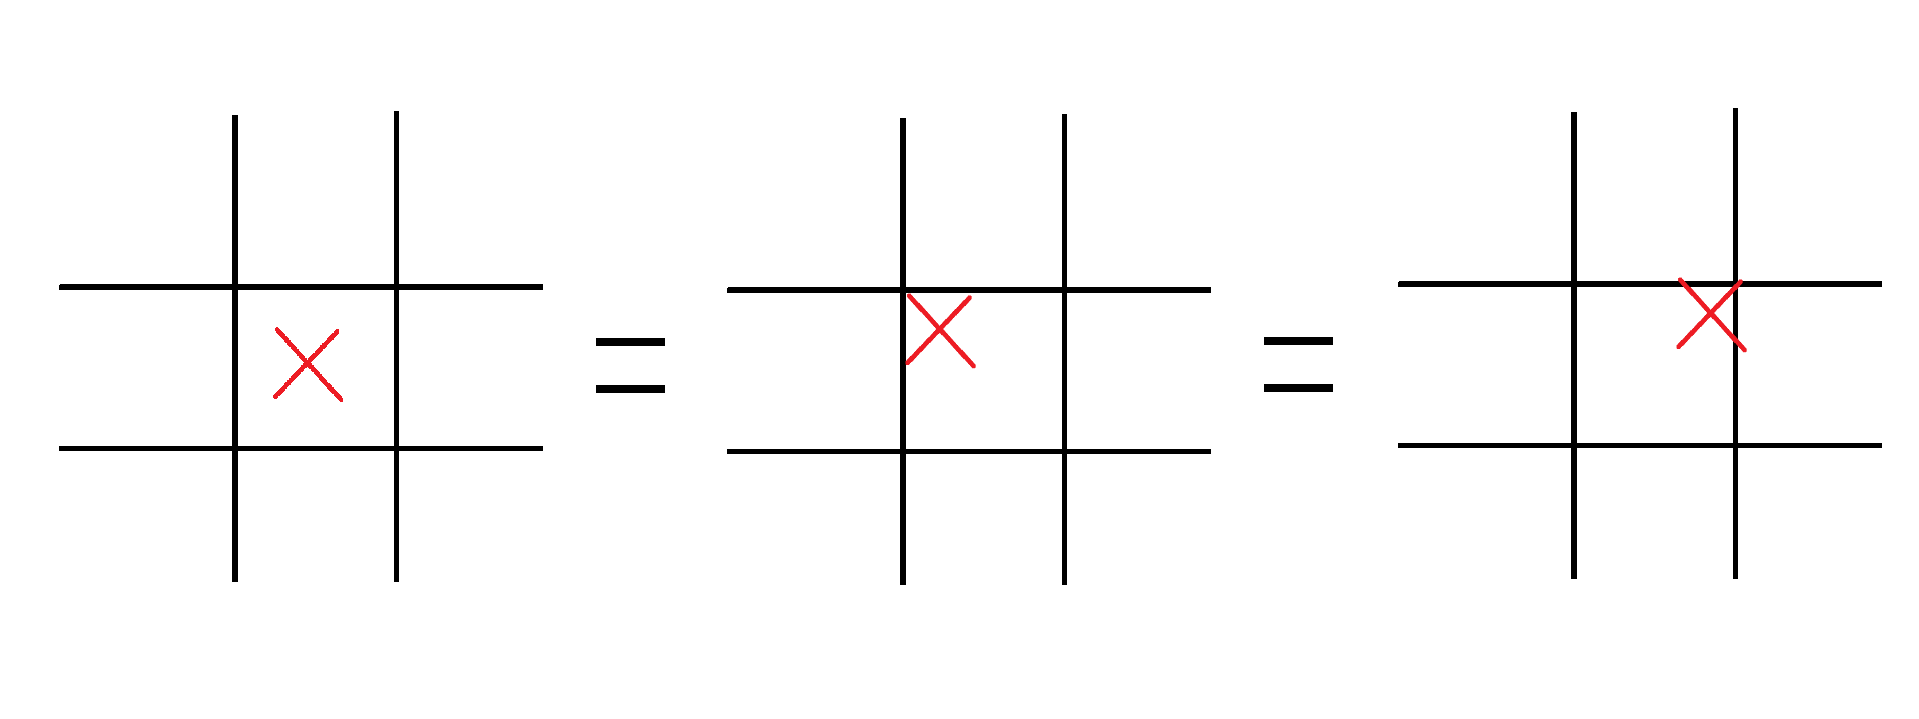
\includegraphics[scale=0.3]{obr/sudoku.png} % soubor + měřítko (scale)
  \caption{Ekvivalence různých značení sudoku.} % popis obrázku
  \label{sudoku} % definice odkazu na obrázek (pro \ref{})
\end{figure}

Hru monopoly pak můžeme definovat jako příklad jednodimenzionální hry. I když je herní deska vizuálně uspořádána do tvaru čtverce, když odstraníme grafické prvky, můžeme vidět, že hra umožňuje pohyb po jediné řadě políček, propojených v cyklické smyčce. V tomto případě se každé políčko na desce chová jako bod nulové dimenze, ačkoliv vizuálně vypadají některé čtverce odlišně, jejich funkce se neliší.

Herní prostor může také zahrnovat „prostory v prostorech“, což se často vyskytuje v počítačových hrách. Například může existovat venkovní prostor (kontinuální, dvourozměrný), ale hráč může narazit na ikony, které představují města nebo jeskyně. Tyto ikony přecházejí do zcela oddělených prostorů, které s venkovním prostorem nejsou přímo propojené, což je příkladem prostorového uspořádání, které je více založeno na mentálních modelech hráčů než na geografické realitě.

\subsubsection{Návrh herního prostoru}

Jak jsem již zmínil, navrhovaná hra bude 2D tahová strategie, tedy herní prostor bude dvoudimenzionální a diskrétní, složený ze čtvercových políček propojených po horizontální a vertikální ploše. To bude mít zásadní vliv na pohyb jednotek po mapě a tedy i veškerá strategická rozhodnutí hráčů.

Diskrétnost herního prostoru usnadňuje měření vzdáleností, po které se jednotky mohou po desce pohybovat, a také omezuje rozložení budov na jednu budovu na políčko. Stejně tak pro jednotky, což umožňuje strategické tahy, jako blokování pohybu jednotek nepřítele.

Ve hře nebudou žádné podprostory ani oblasti, které by hráči mohli navštívit jako separátní oblasti. Celý herní prostor tvoří jednotnou plochu bez vnitřních "meziprostorů" nebo propojení do nových sekcí. Všechny interakce probíhají na jednom herním poli, přičemž všechny herní mechaniky se soustředí na strategické využití této plochy.

Z hlediska návrhu a pozdější implementace tedy herní prostor uvažuji jako dvourozměrné diskrétní pole, kde každé "políčko" představuje bod s nulovou dimenzí. Tento pohled by měl zjednodušit návrh pravidel a interakcí mezi hráči a prostředím, což umožňuje efektivnější rozvoj herních taktik.

\subsubsection{Shrnutí prostoru}

Herní pole tedy pro účely návrhu uvažuji jako abstraktní dvoudimenzionální diskrétní prostor složený z políček propojených na ose $x$ a $y$. Hráči tedy budou moci pohybovat jednotkami pouze ve vertikálním či horizontálním směru, ne diagonálně. Prostor bude jasně vymezen hranicemi (konec vygenerované mapy) a všechny interakce mezi hráči budou probíhat na herní ploše. 

\subsection{Objects, Attributes, and States (Objekty, atributy a stavy)}
\begin{itemize}
    \item Herní entity a jejich stavy:
    \begin{itemize}
        \item Dlaždice (Typy terénů, Stavy dlaždic)
        \begin{itemize}
            \item Typy terénu a jejich vlastnosti
            \item Stav dlaždice -- obsazená, zastavěná
        \end{itemize}
        \item Jednotky
        \begin{itemize}
            \item Typ jednotky -- vlastnosti (pohyb, útok, obrana, speciální schopnosti)
            \item Stavy jednotek -- zraněná, pracuje, ...
        \end{itemize}
        \item Budovy (produkce, obranné stavby, speciální budovy).
        \begin{itemize}
            \item Vlastnosti budov -- cena, produkce
            \item Speciální akce budov
        \end{itemize}
    \end{itemize}
\end{itemize}

\subsection{Actions (Akce hráče)}
\begin{itemize}
    \item Možné akce hráče během tahu:
    \begin{itemize}
        \item Pohyb jednotek. (Použití speciálních schopností jednotek)
        \item Útok a bojový systém. 
        \item Stavba budov a infrastruktury. (Správa zdrojů a ekonomika)
    \end{itemize}
\end{itemize}

\subsection{Rules (Pravidla hry)}
\begin{itemize}
    \item Základní pravidla:
    \begin{itemize}
        \item Podmínky vítězství (zničení nepřítele).
        \item Struktura tahu (pořadí akcí).
        \item Omezující pravidla (pohybové limity, ztráta jednotek, zničení budov).
    \end{itemize}
    \item Vyváženost a spravedlnost pravidel.
\end{itemize}

\subsection{Skill and Chance (Dovednost a náhoda)}
\begin{itemize}
    \item Jaký vliv má dovednost hráče na výsledek hry:
    \begin{itemize}
        \item Strategické plánování.
        \item Správné rozhodování a reakce na situace.
    \end{itemize}
    \item Jaký vliv má náhoda:
    \begin{itemize}
        \item Procedurálně generovaná mapa jako faktor variabilních podmínek.
    \end{itemize}
    \item Vyvážení mezi dovedností a náhodou.
\end{itemize}

\subsection{Shrnutí}
\begin{itemize}
    \item Shrnutí hlavních bodů návrhu.
    \item Vztah návrhu k procedurálnímu generování map.
\end{itemize}
